%======================================================================
%  APPENDIX  :  ADDITIONAL BEHAVIOURAL EVIDENCE
%======================================================================
\newpage
\section{Additional behavioral evidence}
\label{app:behaviour}

%----------------------------------------------------------------------
%======================= EXECUTION PACE  =======================
%----------------------------------------------------------------------

\begin{figure}[H]
    \centering
    \captionsetup[subfigure]{justification=centering}
    %---------------------------  CDA  ----------------------------------%
    \begin{subfigure}[t]{\textwidth}
        \centering
        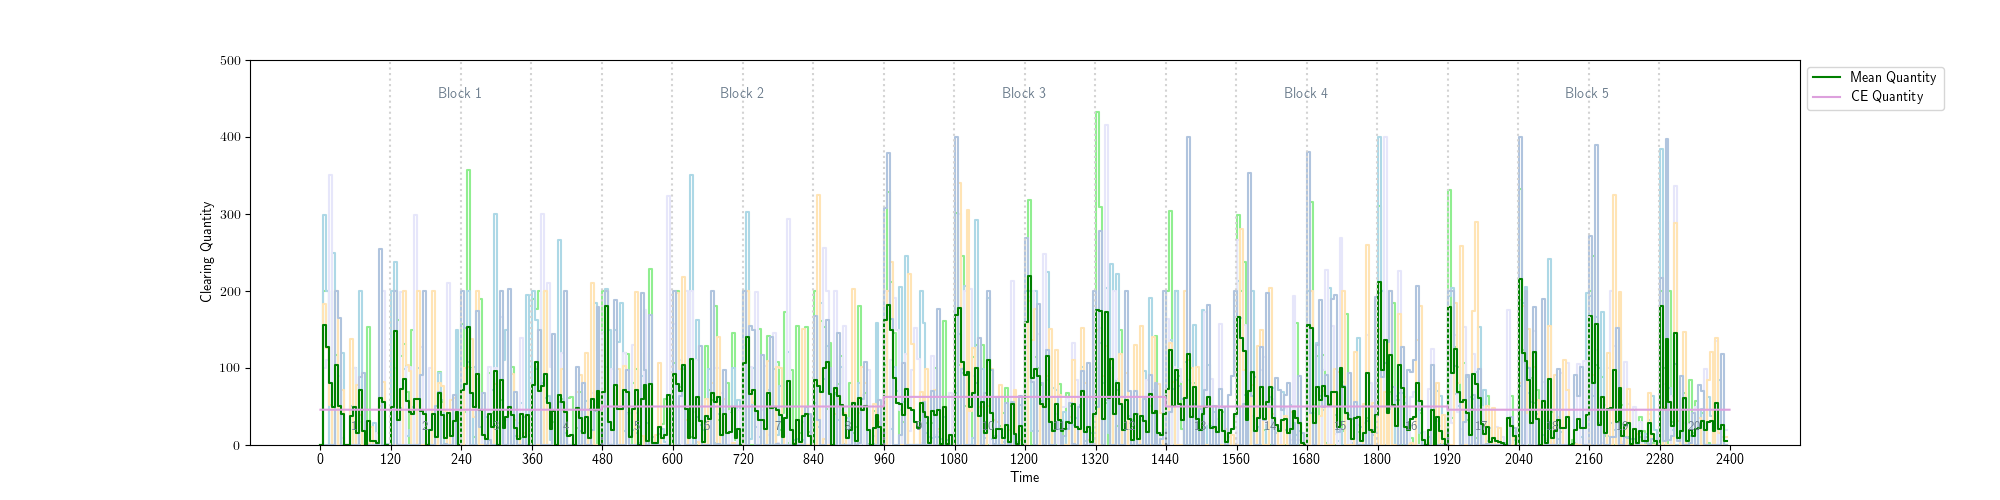
\includegraphics[width=\linewidth]{new plots/groups_cda_rate.png}
        \caption{CDA}
        \label{fig:rate_cda}
    \end{subfigure}\par\medskip
    %---------------------------  FlowR  --------------------------------%
    \begin{subfigure}[t]{\textwidth}
        \centering
        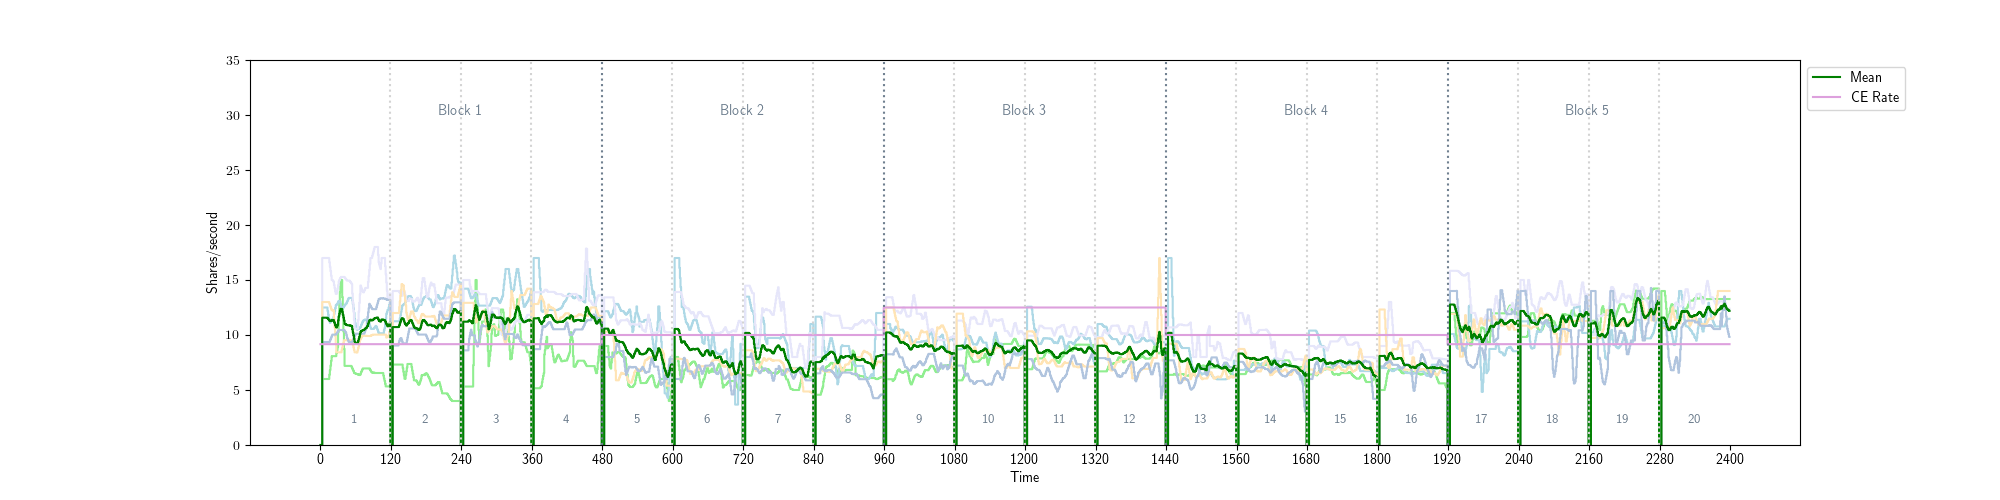
\includegraphics[width=\linewidth]{new plots/groups_flow_rate_r.png}
        \caption{FlowR (cap $=30$\,sh/s)}
        \label{fig:rate_flowr}
    \end{subfigure}\par\medskip
    %---------------------------  FlowS  --------------------------------%
    \begin{subfigure}[t]{\textwidth}
        \centering
        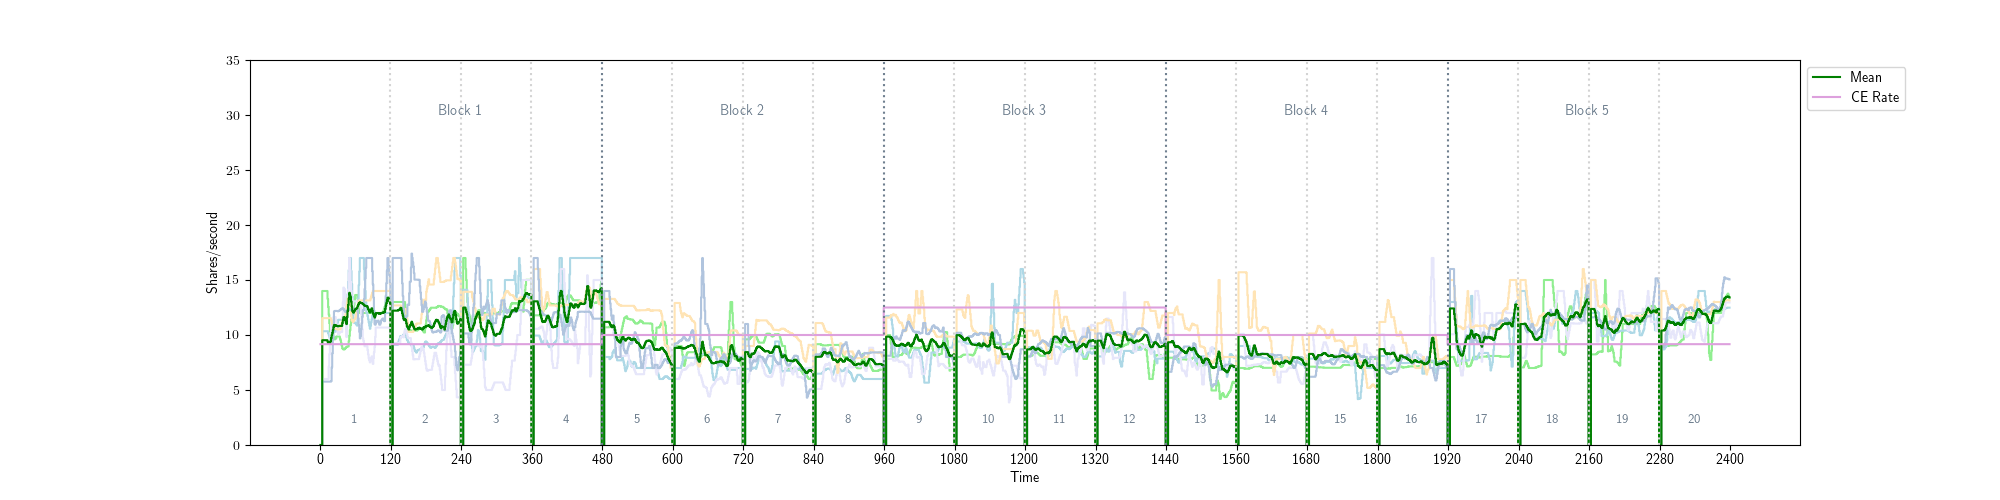
\includegraphics[width=\linewidth]{new plots/groups_flow_rate_s.png}
        \caption{FlowS (cap $=60$\,sh/s)}
        \label{fig:rate_flows}
    \end{subfigure}
    \caption{\textbf{Mean execution pace (shares per second).}  
             Each panel traces the average rate over the
             trading window. For CDA this is calculated in intervals of five seconds. The pink lines are the predicted CE pace.}
    \label{fig:execution_rates_detailed}
\end{figure}









%----------------------------------------------------------------------
%=======================  Scatter : max–rate usage vs. realised surplus
%----------------------------------------------------------------------
\begin{figure}[H]
    \centering
    \begin{adjustbox}{trim=0 0 0 {.0\height},clip=true}
        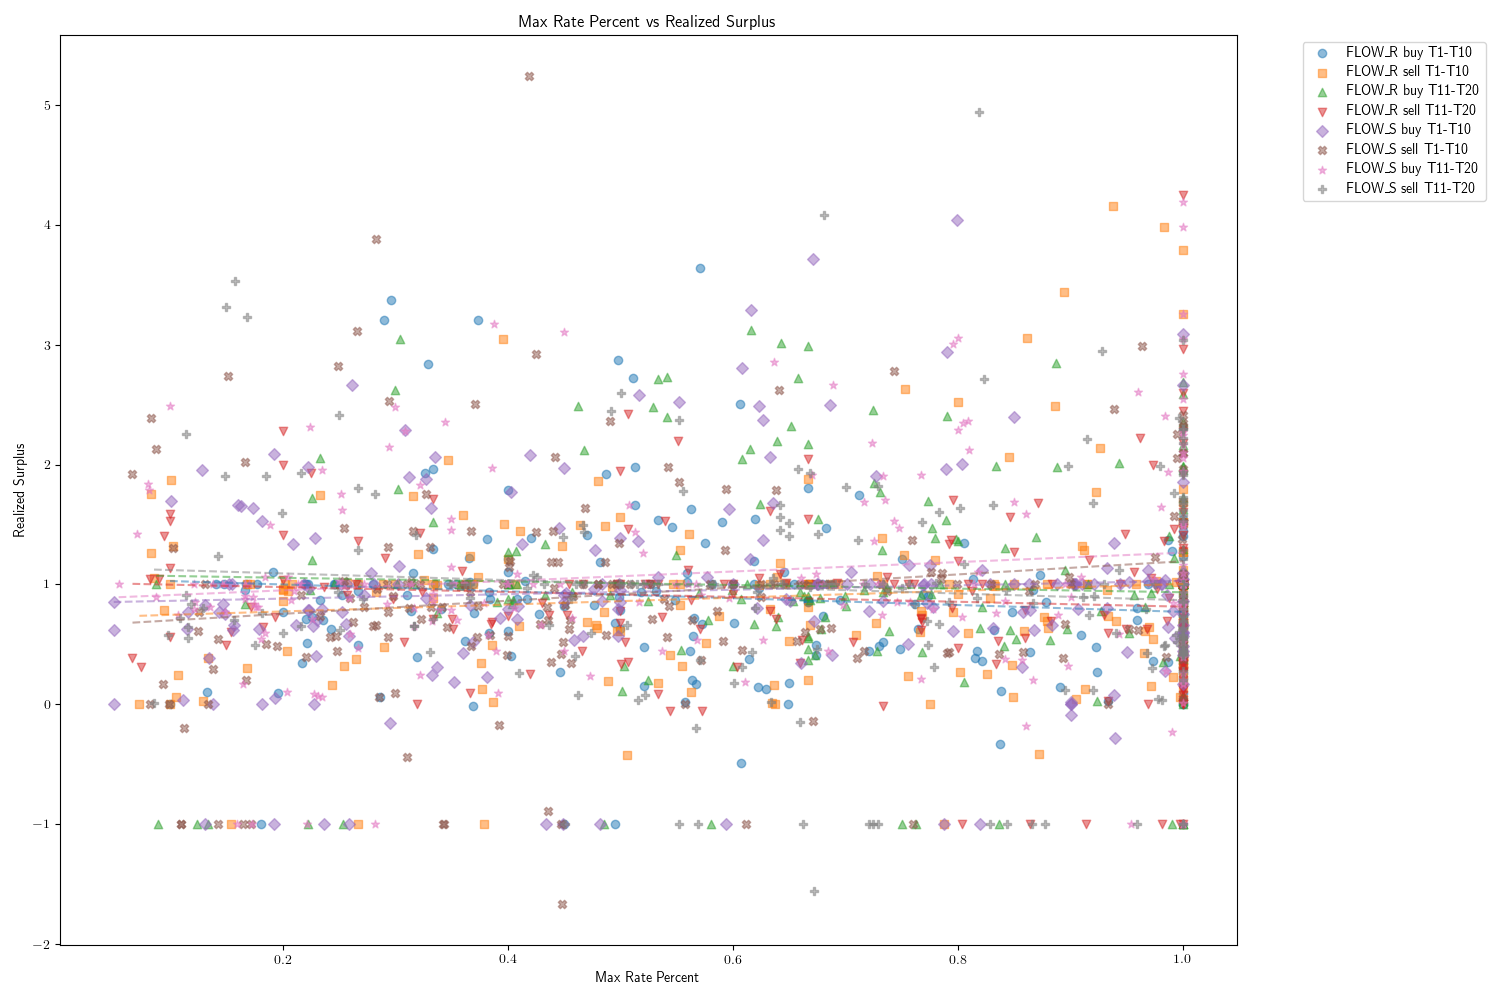
\includegraphics[width=.78\linewidth]{new plots/groups_flow_max_rate_percent_vs_realized_surplus.png}
    \end{adjustbox}
    \caption{Scatter of the share of the speed limit used
             ($U_{\max}/U_{\max}^{\text{limit}}$) against realised
             surplus. Break down by market side (buyer vs.\ seller) and
             by Flow variant (R vs.\ S) and first/second session half. Fitted lines are OLS slopes.}
    \label{fig:scatter_maxrate_realsurplus}
\end{figure}




%----------------------------------------------------------------------
%=======================  table: correlations
%----------------------------------------------------------------------

\begin{table}[H]
\centering
\caption{Correlations Between Behavioral Variables (group–level averages)}
\label{tab:correlations-appendix}
% \scriptsize
\setlength{\tabcolsep}{5pt}
\begin{threeparttable}
\begin{tabular}{@{}lcccccc@{}}
\toprule
 % & \multicolumn{1}{c}{EP\,vs.\,$P-dev$} & \multicolumn{1}{c}{EP\,vs.\,MRate\%} & \multicolumn{1}{c}{EP\,vs.\,$\Delta P$} & \multicolumn{1}{c}{$\Delta p$\,vs.\,MRate} & \multicolumn{1}{c}{$\Delta p$\,vs.\,$\Delta P$} & \multicolumn{1}{c}{$\Delta P$\,vs.\,Rate\%} \\
 & \multicolumn{1}{c}{\begin{tabular}[c]{@{}c@{}}EP vs.\\$P\text{-dev}$\end{tabular}} 
& \multicolumn{1}{c}{\begin{tabular}[c]{@{}c@{}}EP vs.\\MRate\,(\%)\end{tabular}} 
& \multicolumn{1}{c}{\begin{tabular}[c]{@{}c@{}}EP vs.\\$\Delta P$\end{tabular}} 
& \multicolumn{1}{c}{\begin{tabular}[c]{@{}c@{}}$P\text{-dev}$ vs.\\MRate\,(\%)\end{tabular}} 
& \multicolumn{1}{c}{\begin{tabular}[c]{@{}c@{}}$P\text{-dev}$ vs.\\$\Delta P$\end{tabular}} 
& \multicolumn{1}{c}{\begin{tabular}[c]{@{}c@{}}$\Delta P$ vs.\\MRate\,(\%)\end{tabular}} \\
\midrule
\multicolumn{7}{@{}l}{\textit{FlowR — Buyers}} \\
\quad T1–T10  & -0.022 & -0.306 & -0.058 &  0.133 & -0.004 & -0.371 \\
\quad T11–T20 &  0.141 & -0.195 &  0.119 & -0.108 & -0.024 & -0.333 \\[4pt]
\multicolumn{7}{@{}l}{\textit{FlowR — Sellers}} \\
\quad T1–T10  &  0.350 & -0.029 &  0.070 &  0.110 & -0.054 &  0.286 \\
\quad T11–T20 &  0.005 & -0.103 &  0.006 &  0.100 & -0.039 &  0.249 \\[4pt]
\multicolumn{7}{@{}l}{\textit{FlowS — Buyers}} \\
\quad T1–T10  & -0.036 &  0.083 &  0.170 & -0.104 & -0.160 &  0.238 \\
\quad T11–T20 & -0.275 &  0.109 &  0.279 & -0.206 & -0.077 &  0.097 \\[4pt]
\multicolumn{7}{@{}l}{\textit{FlowS — Sellers}} \\
\quad T1–T10  & -0.034 &  0.193 & -0.130 & -0.144 & -0.043 & -0.222 \\
\quad T11–T20 &  0.094 & -0.066 &  0.173 & -0.126 &  0.237 & -0.213 \\
\bottomrule
\end{tabular}
\begin{tablenotes}[flushleft]
\footnotesize
\item \textit{Notes:} EP = Excess profit; $P-dev$ = Price deviation from contract price; $\Delta P$ = Price range ($p_H-p_L$); MRate = Chosen maximum rate. All coefficients are Spearman correlations computed at the group level.
% KL: ask Yilin about the level of this calculation 
\end{tablenotes}
\end{threeparttable}
\end{table}




% =============== Scatter plots

\begin{figure}[H]
    \centering
    \captionsetup[subfigure]{justification=centering}
    %---------------------  (a) Price‐range width vs. profit  --------------------%
    \begin{subfigure}[t]{0.65\textwidth}
        \centering
        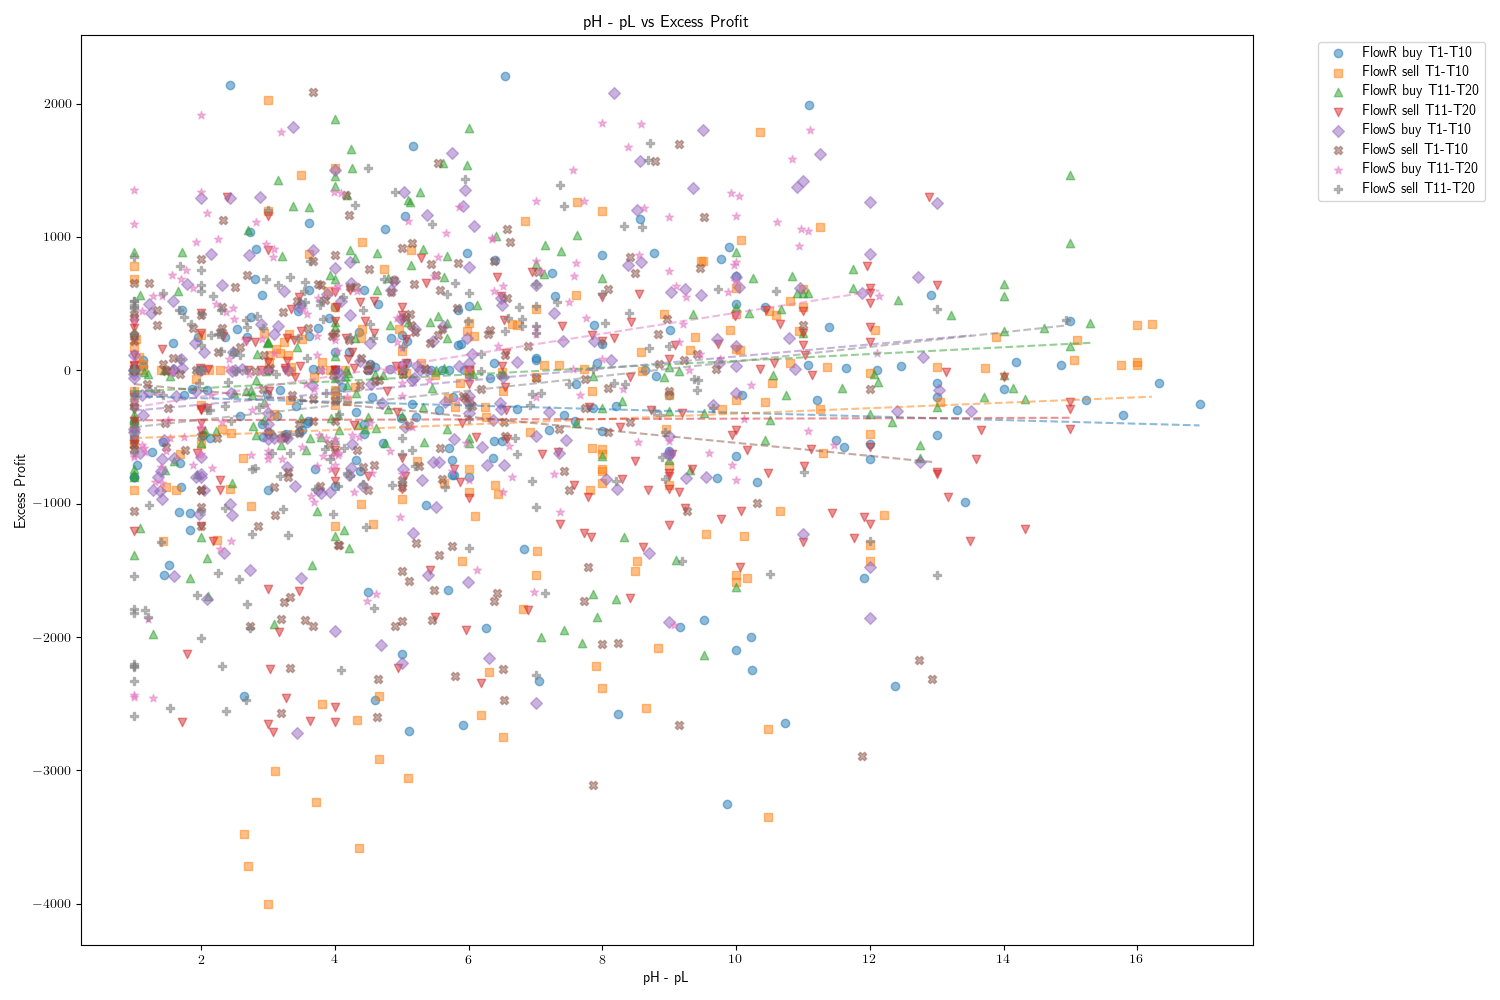
\includegraphics[width=.85\textwidth]{new plots/groups_flow_pH-pL_vs_excess_profit.png}
        \caption{Price‐range width ($p_H\!-\!p_L$) against excess profit.}
        \label{fig:range_profit}
    \end{subfigure}\par\medskip
    %---------------------  (b) Max-rate share vs. profit  -----------------------%
    \begin{subfigure}[t]{0.65\textwidth}
        \centering
        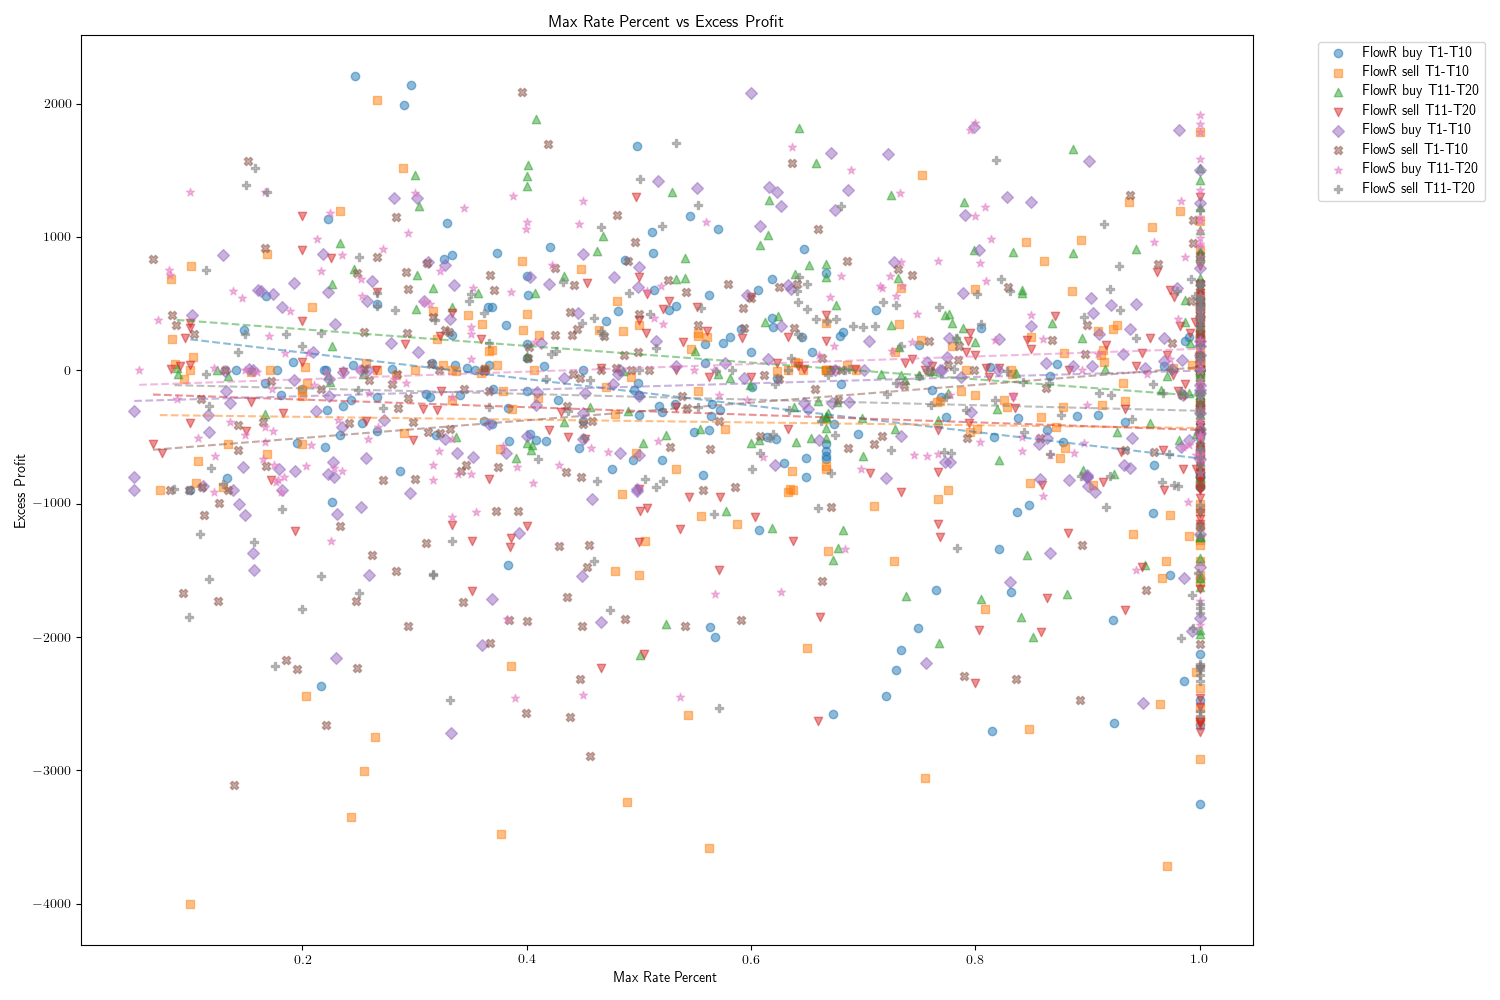
\includegraphics[width=.85\textwidth]{new plots/groups_flow_max_rate_percent_vs_excess_profit.png}
        \caption{Chosen maximum rate as a percentage of the cap vs.\ excess profit.}
        \label{fig:rate_profit}
    \end{subfigure}\par\medskip
    %---------------------  (c) Price deviation vs. profit  ----------------------%
    \begin{subfigure}[t]{0.65\textwidth}
        \centering
        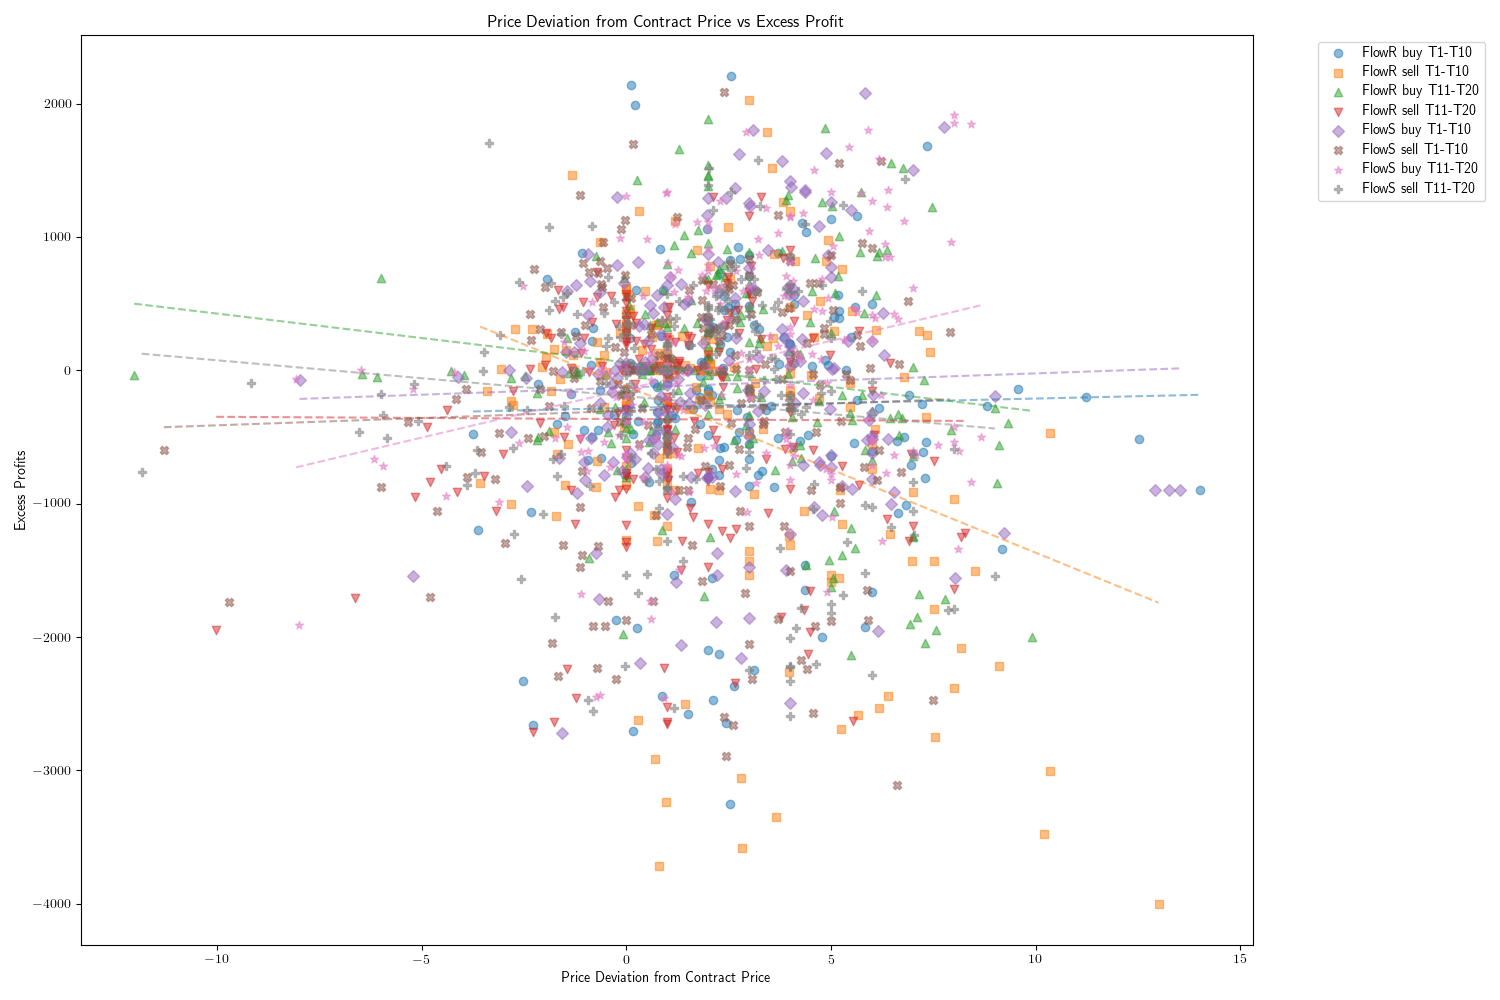
\includegraphics[width=.85\textwidth]{new plots/groups_flow_price_dev_from_contract_vs_excess_profit.png}
        \caption{Price deviation from contract ($\Delta p$) against excess profit.}
        \label{fig:dev_profit}
    \end{subfigure}
    \caption{\textbf{Behavioral levers and realised surplus.}  
             Each panel scatters show a variable against excess
             profit at the trader level.}
    % \label{fig:lever_profit}
    \label{fig:app_excess-profit-correlations}
\end{figure}



%%%%%%%%%%%%%%%%%%%%%%%%%%%%%%%%%%%%%%%%%%%%%%%%%%%%%%%%%%%%%%%%%%%%%%%%%%%%%%%%%%%%%%%%%%%%%%%%%%%%%%%%%%%%%%%%%%%%%%%%%%%%%%%%%%%%%%%%%%%%%%%%%%%%%%%%%%%%%%%%%%%%%%%%%%%%%%%%%%%%%%%%%%%%%%%%%%%%%%%%%%%%%%%%%%%%%%%%%%%%%%%%%%%%%%%%%%%%%%%%%%%%%%%%%%%%%%%%%%%%%%%%%%%%%%%%%%%%%%%%%%%%%%%%%%%%%%%%%%%%%%%%%%%%%%%%%%%%%%%%%%%%%%%%%%%%%%%%%%%%%%%%%%%%%%%%%%%%%%%%%%%%%%%%%%%%%%%%%%%%%%%%%%%%%%%%%%%%%%%%%%%%%%%%%%%%%%%%%%%%%%%%%%%%%%%%%%%%%%%%%%%%


%=======================  REALISED SURPLUS TRAJECTORIES  

\begin{figure}[H]
    \centering
    \captionsetup[subfigure]{justification=centering}
    %---------------------------  CDA  ----------------------------------%
    \begin{subfigure}[t]{\textwidth}
        \centering
        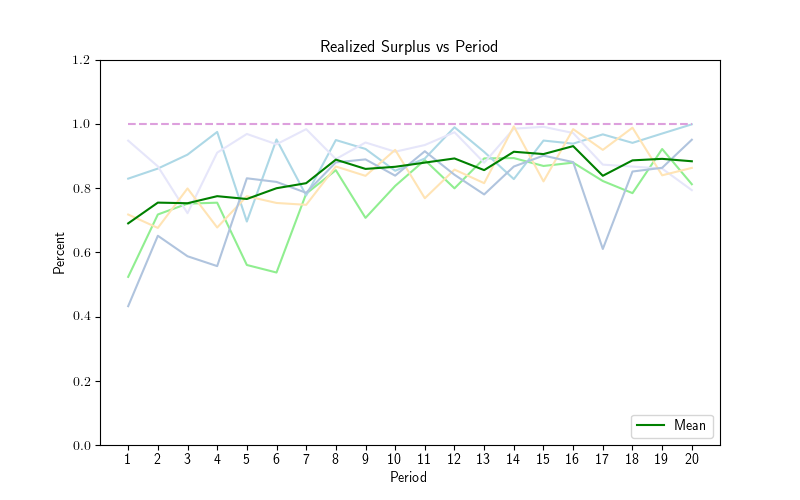
\includegraphics[width=\linewidth]{new plots/groups_cda_surplus.png}
        \caption{CDA}
        \label{fig:surplus_cda}
    \end{subfigure}\par\medskip
    %---------------------------  FlowR  --------------------------------%
    \begin{subfigure}[t]{\textwidth}
        \centering
        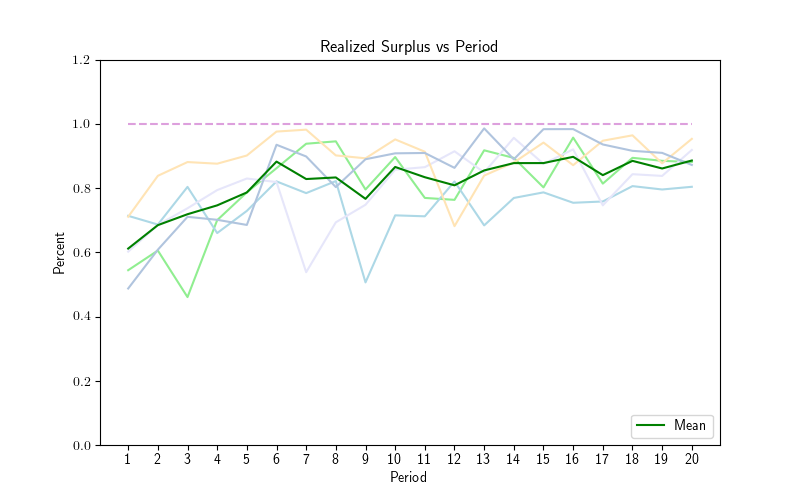
\includegraphics[width=\linewidth]{new plots/groups_flow_surplus_r.png}
        \caption{FlowR (cap $=30$\,sh/s)}
        \label{fig:surplus_flowr}
    \end{subfigure}\par\medskip
    %---------------------------  FlowS  --------------------------------%
    \begin{subfigure}[t]{\textwidth}
        \centering
        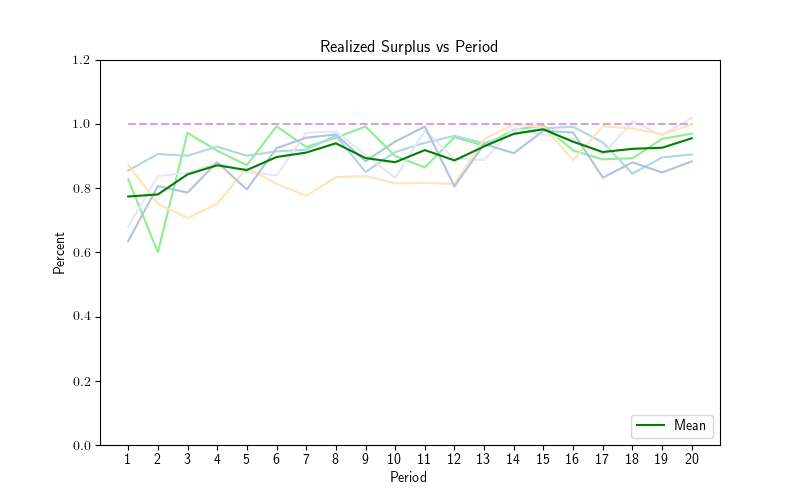
\includegraphics[width=\linewidth]{new plots/groups_flow_surplus_s.png}
        \caption{FlowS (cap $=60$\,sh/s)}
        \label{fig:surplus_flows}
    \end{subfigure}
    \caption{\textbf{Cumulative realised surplus relative to the competitive benchmark.}  
             Lines plot the running total of profits (in ECU) as a
             percentage of the competitive‐equilibrium surplus.  Both
             Flow variants outperform CDA, with FlowS overtaking FlowR
             after period~10, consistent with the learning dynamics
             discussed in Section~\ref{sec:flow-behaviour}.  Error bars
             denote $\pm1$ standard errors across groups.}
    \label{fig:surplus_trajectories}
\end{figure}



%===========================================================
%  Realised–surplus distributions (three panels)
%===========================================================
\begin{figure}[t]
    \centering
    %-------------------- CDA --------------------%
    \begin{subfigure}[b]{.32\linewidth}
        \centering
        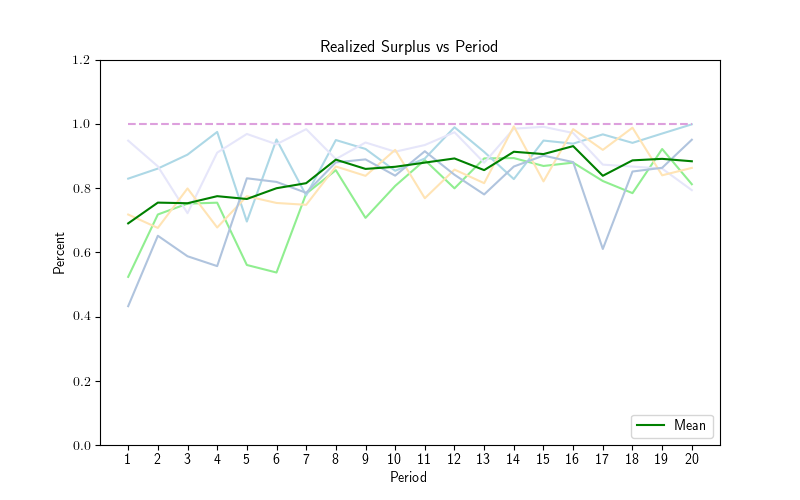
\includegraphics[width=\linewidth]{new plots/groups_cda_surplus.png}
        \subcaption{\tiny CDA (benchmark)}
    \end{subfigure}%
    %-------------------- FlowR --------------------%
    \begin{subfigure}[b]{.32\linewidth}
        \centering
        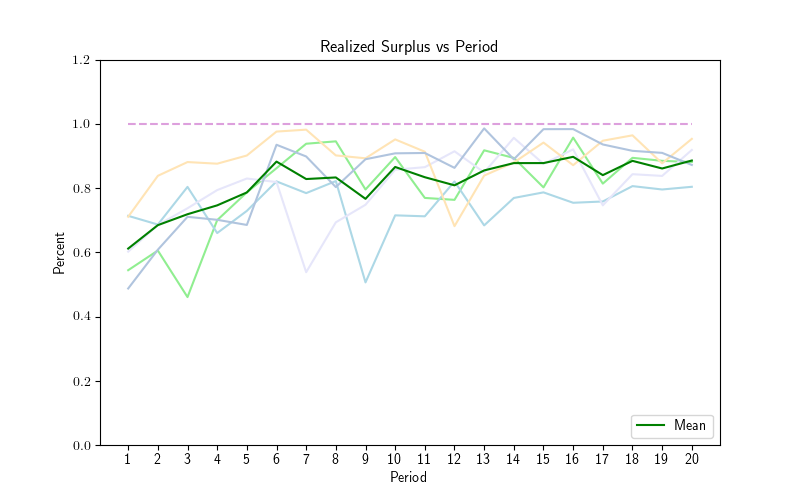
\includegraphics[width=\linewidth]{new plots/groups_flow_surplus_r.png}
        \subcaption{\tiny FlowR ($U_{\max}=30$)}
    \end{subfigure}%
    %-------------------- FlowS --------------------%
    \begin{subfigure}[b]{.32\linewidth}
        \centering
        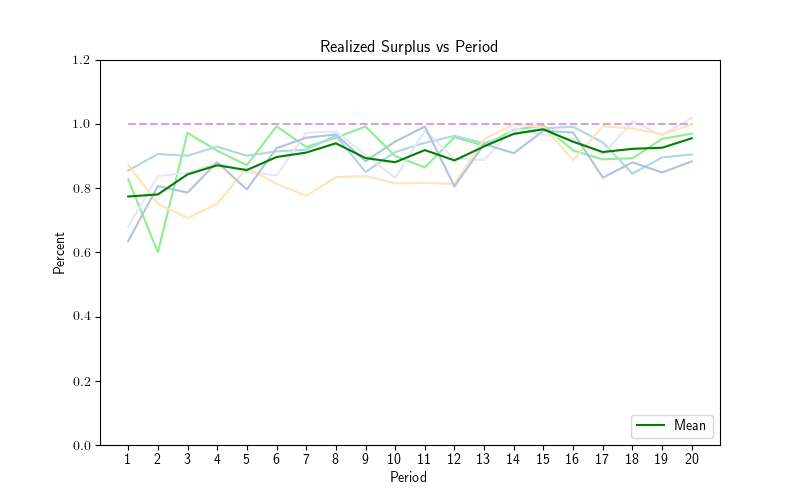
\includegraphics[width=\linewidth]{new plots/groups_flow_surplus_s.png}
        \subcaption{\tiny FlowS ($U_{\max}=60$)}
    \end{subfigure}
    \caption{Distribution of realised surplus as a fraction of the competitive-equilibrium surplus.  Both Flow formats shift the entire distribution to the right relative to CDA, with FlowS exhibiting the largest efficiency gains.}
    \label{fig:surplus-dist}
\end{figure}



%======================  REALISED SURPLUS TRAJECTORIES  ======================
\begin{figure}[H]
    \centering
    \captionsetup[subfigure]{justification=centering}
    %---------------------------  CDA  ----------------------------------%
    \begin{subfigure}[t]{.32\linewidth}
        \centering
        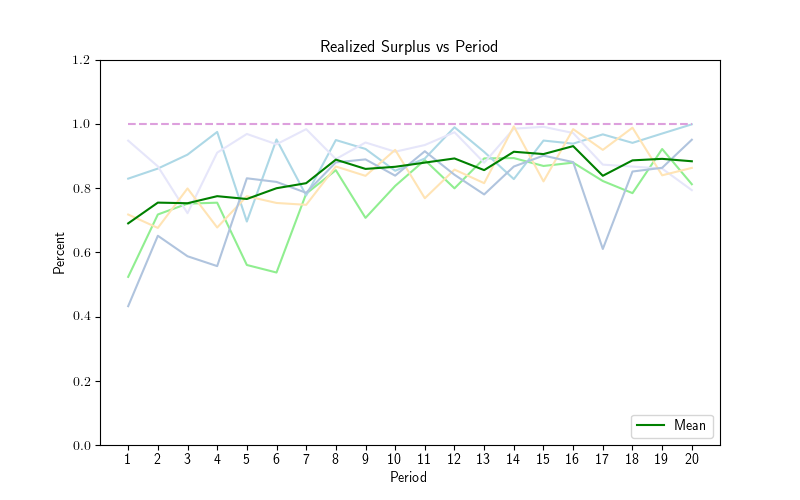
\includegraphics[width=\linewidth]{new plots/groups_cda_surplus.png}
        \caption{CDA}
        \label{fig:surplus_cda}
    \end{subfigure}
    \hfill
    %---------------------------  FlowR  --------------------------------%
    \begin{subfigure}[t]{.32\linewidth}
        \centering
        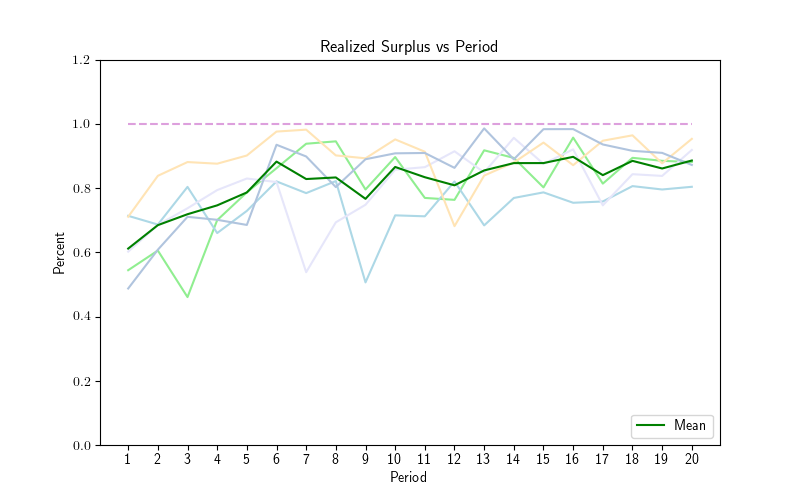
\includegraphics[width=\linewidth]{new plots/groups_flow_surplus_r.png}
        \caption{FlowR \\ (cap $=30$\,sh/s)}
        \label{fig:surplus_flowr}
    \end{subfigure}
    \hfill
    %---------------------------  FlowS  --------------------------------%
    \begin{subfigure}[t]{.32\linewidth}
        \centering
        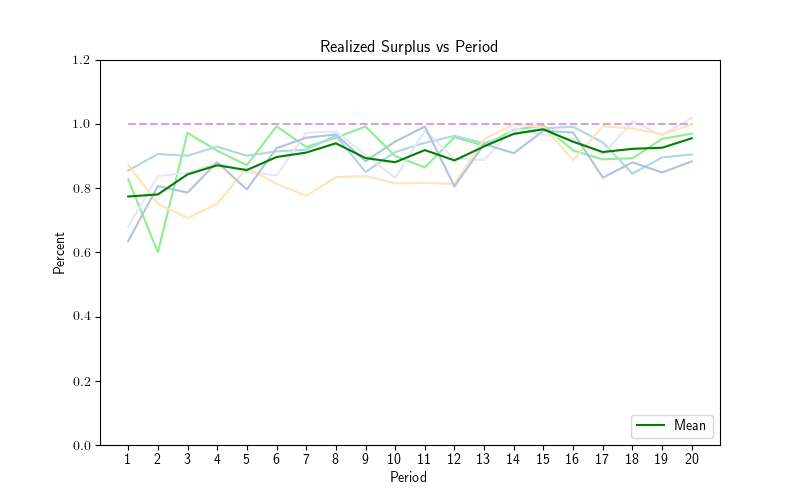
\includegraphics[width=\linewidth]{new plots/groups_flow_surplus_s.png}
        \caption{FlowS \\ (cap $=60$\,sh/s)}
        \label{fig:surplus_flows}
    \end{subfigure}
    \caption{\textbf{Cumulative realised surplus relative to the competitive benchmark.}  
             Lines plot the running total of profits (in ECU) as a
             percentage of the competitive-equilibrium surplus.  Both
             Flow variants outperform CDA, with FlowS overtaking FlowR
             after period~10, consistent with the learning dynamics
             discussed in Section~\ref{sec:flow-behaviour}.  Error bars
             denote $\pm1$ standard errors across groups.}
    \label{fig:surplus_trajectories}
\end{figure}

